\setlength{\columnsep}{3pt}
\begin{flushleft}

		\begin{itemize}
	\item \textbf{Single-core processors}: 
	\begin{itemize}
		\item A single CPU with \textbf{one core}.
		\item Can execute only one command at a time.
		\item It is not efficient in multi-tasking.
		\begin{figure}[h!]
			\centering
			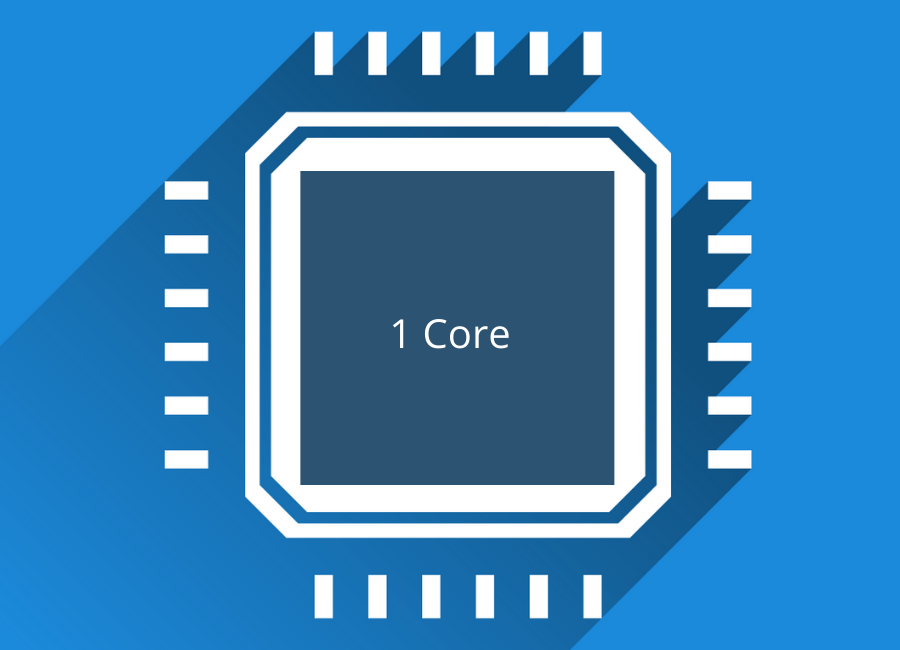
\includegraphics[scale=.3]{content/chapter12/images/single.png}
			\caption{Single-core CPU}
			\label{fig:single-core1}
		\end{figure}
	\end{itemize}
	
	\bigskip
	
	\item \textbf{Dual-core(2 cores) processors}:
	\begin{itemize}
		\item A single CPU with \textbf{two cores}.
		\item Functions like dual CPU acting like one. 
		\begin{figure}[h!]
			\centering
			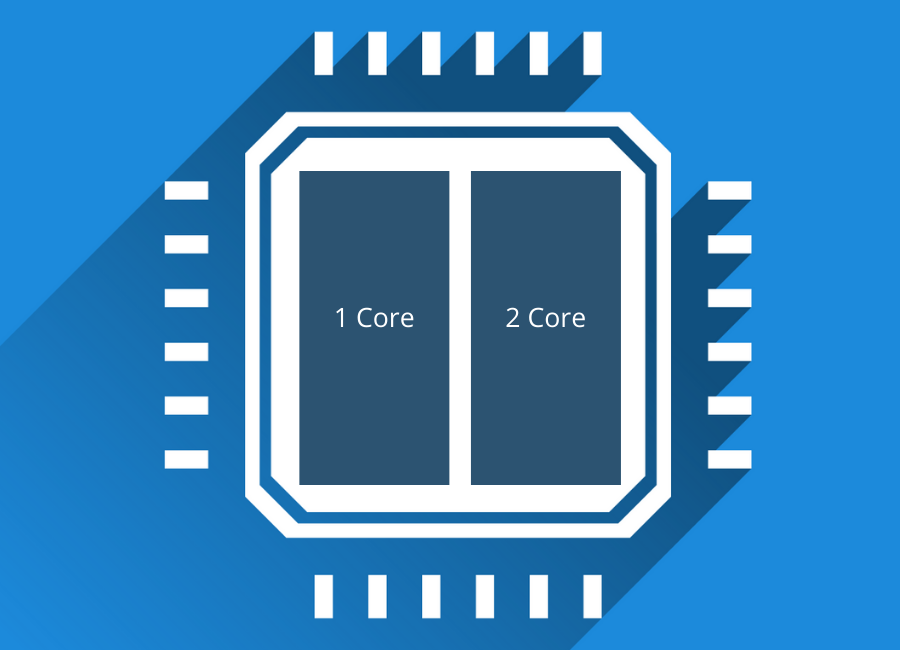
\includegraphics[scale=.3]{content/chapter12/images/dual.png}
			\caption{Dual-core CPU}
			\label{fig:single-core2}
		\end{figure}
	\end{itemize}
	\newpage
	\item \textbf{Quad-core(4 cores) processors}:
	\begin{itemize}
		\item The quad-core CPU comes with \textbf{four cores} on a single CPU. 
		\item Such types of CPU are used by gamers.
		\begin{figure}[h!]
			\centering
			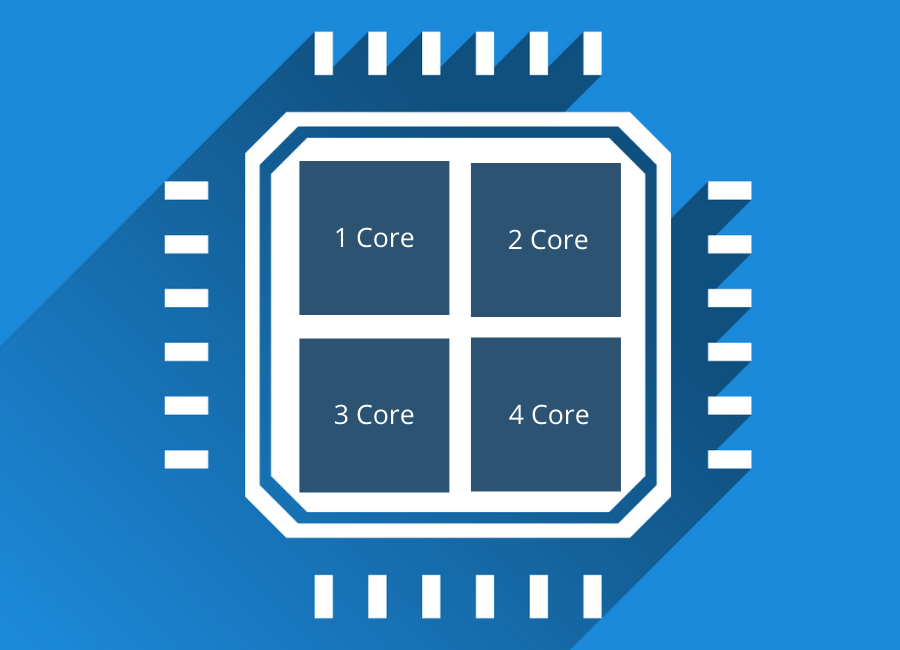
\includegraphics[scale=.3]{content/chapter12/images/quad.png}
			\caption{Quad-core CPU}
			\label{fig:single-core3}
		\end{figure}
	\end{itemize}			
	
	\bigskip
	
	\item \textbf{Hexa Core(6 cores) processors}:
	\begin{itemize}
		\item The hexa-core CPU comes with \textbf{six cores} on a single CPU. 
		\item Intel has launched with Inter core i7 in 2010 with Hexa core processor.
		\begin{figure}[h!]
			\centering
			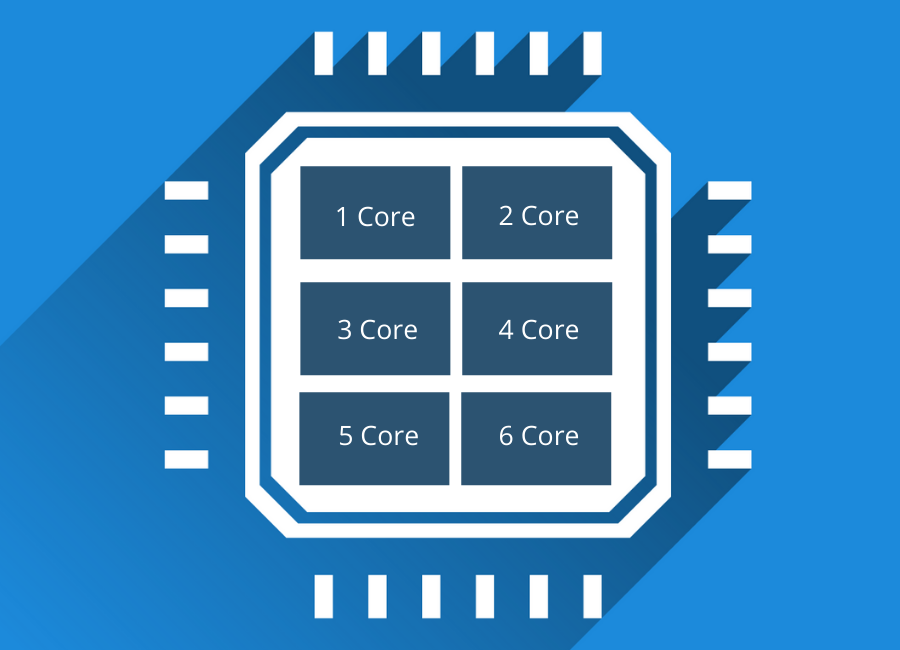
\includegraphics[scale=.3]{content/chapter12/images/hexa.png}
			\caption{Hexa-core CPU}
			\label{fig:single-core4}
		\end{figure}
	\end{itemize}			
	\newpage
	\item \textbf{Octa Core(8 cores) processors}:
	\begin{itemize}
		\item It is multiple core processor with 8 cores.
		\item For gaming, video editing, and other processor-intensive applications, eight cores or more is ideal.
		\begin{figure}[h!]
			\centering
			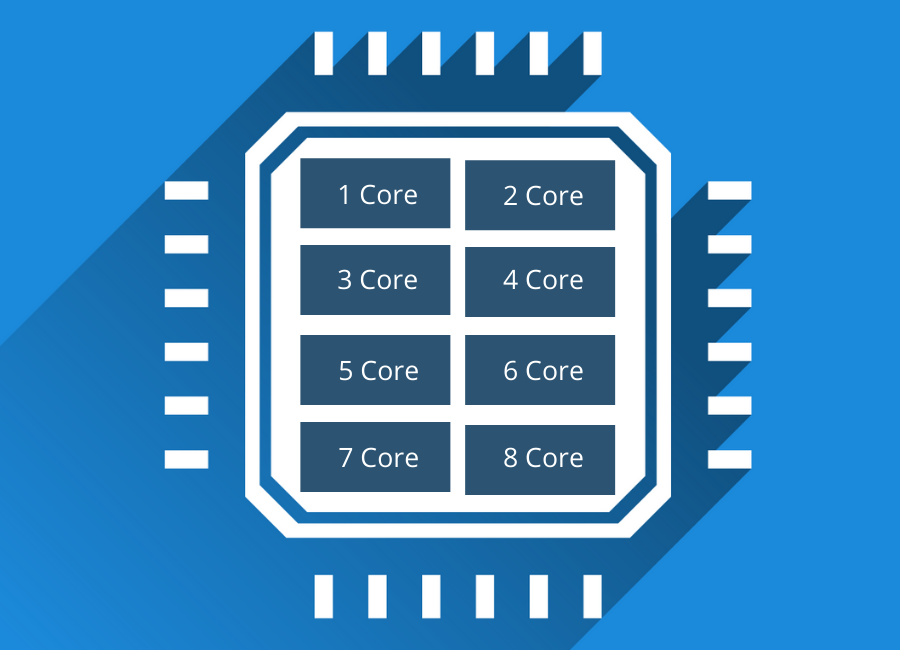
\includegraphics[scale=.3]{content/chapter12/images/octa.png}
			\caption{Octa-core CPU}
			\label{fig:single-core4}
		\end{figure}
	\end{itemize}		
	
	\bigskip
	
	\item \textbf{Deca-Core(10 cores) processors}:
	\begin{itemize}
		\item It is multiple core processor with 10 cores.
		\item Iideal for gamers and users who do heavy multitasking.
		\begin{figure}[h!]
			\centering
			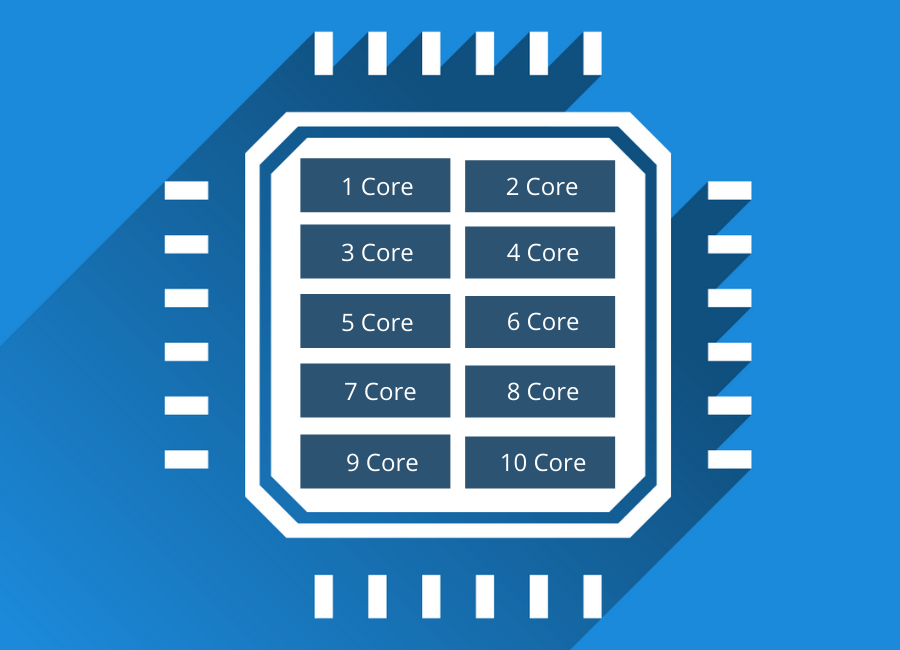
\includegraphics[scale=.3]{content/chapter12/images/deca.png}
			\caption{Deca-core CPU}
			\label{fig:single-core4}
		\end{figure}
	\end{itemize}		
	
	
\end{itemize}

\end{itemize}



\end{flushleft}

\newpage


